\documentclass[
    10pt,
    aspectratio=169,
    usenames,
    dvipsnames
]{beamer}
% As the Metropolis theme this theme is licensed under a Creative Commons Attribution-ShareAlike 4.0 International License. This means that if you change the theme and re-distribute it, you must retain the copyright notice header and license it under the same CC-BY-SA license. This does not affect the presentation that you create with the theme.
\usetheme{metropolis}
\usepackage{xargs}

\definecolor{bimosred}{HTML}{A60000}
\definecolor{bimosyellow}{HTML}{FFFFFF}  % TU light gray
\definecolor{bimosblack}{HTML}{23373B}  % Very dark version of TU gray-blue.

\setbeamercolor{normal text}{fg=bimosblack!95!bimosyellow, bg=bimosyellow}

% {bimosred!75!normal text.fg} is the average color of the BIMoS logo in the footer.
\setbeamercolor{frametitle}{fg=bimosred!75!normal text.fg, bg=normal text.bg}
\setbeamercolor{footline}{fg=bimosred!75!normal text.fg}
\setbeamercolor{alerted text}{fg=bimosred!95!bimosyellow}
\setbeamercolor{example text}{fg=bimosblack!75!bimosyellow}
\setbeamercolor{block title alerted}{fg=bimosred!95!bimosyellow}

\newcommand{\bimos}{\textbf{BIMoS}\xspace}
% \newcommandx{\foo}[3][1=1, 3=n]{...}
\newcommandx{\bimostitle}[3][2=0pt, 3=0pt]{\par\vspace{#2}\hspace{-4ex}\textcolor{frametitle.fg}{\large \textbf{#1}}\par\vspace{#3}}


\metroset{block=fill}

\makeatletter % Override @ meaning
\define@key{beamerframe}{standout}[true]{%
  \booltrue{metropolis@standout}
  \begingroup
    \setkeys{beamerframe}{c}
    \setkeys{beamerframe}{noframenumbering}
    \setbeamercolor{background canvas}{
        use=normal text,
        bg=normal text.fg
    }
    \setbeamertemplate{footline}{}
    \setbeamercolor{local structure}{
      use=normal text,
      fg=normal text.bg
    }
    \usebeamercolor[bg]{normal text}
}
  \pretocmd{\beamer@reseteecodes}{%
    \ifbool{metropolis@standout}{
      \endgroup
      \boolfalse{metropolis@standout}
    }{}
  }{}{}
  \AtBeginEnvironment{beamer@frameslide}{
    \ifbool{metropolis@standout}{
      \centering
      \usebeamerfont{standout}
    }{}
  }

% \setbeamertemplate{frame footer}{\insertshortauthor\hfill\textbf{BIMoS}}
% \setbeamertemplate{footline}[plain]
\defbeamertemplate{footline}{bimos}{
  \begin{beamercolorbox}[wd=\textwidth, sep=2ex]{footline}%
    \usebeamerfont{page number in head/foot}%
    \parbox[b]{0.43\textwidth}{\hspace*{1ex}\insertshortauthor}
    %\parbox[b]{0.10\textwidth}{\centering\vspace{0.2ex}\includegraphics[height=0.775em]{bimos-logo2.png}\vspace{-0.2ex}} % \textbf{BIMoS}}
    \parbox[b]{0.53\textwidth}{\hfill
    \usebeamertemplate*{frame numbering}}
  \end{beamercolorbox}%
}
\makeatother % End override
\setbeamertemplate{footline}[bimos]
\setbeamertemplate{title graphic}{
    \inserttitlegraphic
    \vspace{3mm}
}
\setbeamertemplate{title page}{
  \begin{minipage}[b][\paperheight]{\textwidth}
    \vfill
    \ifx\inserttitle\@empty\else\usebeamertemplate*{title}\fi
    \ifx\insertsubtitle\@empty\else\usebeamertemplate*{subtitle}\fi
    \usebeamertemplate*{title separator}
    \ifx\beamer@shortauthor\@empty\else\usebeamertemplate*{author}\fi
    \ifx\insertdate\@empty\else\usebeamertemplate*{date}\fi
    \ifx\insertinstitute\@empty\else\usebeamertemplate*{institute}\fi
    \vfill
    \ifx\inserttitlegraphic\@empty\else\usebeamertemplate*{title graphic}\fi
    \vspace*{1mm}
  \end{minipage}
}

% Fonts and Encoding
\usepackage[T1]{fontenc}                % Sets font encoding to use 8 bit encoding
\usepackage{lmodern}                    % Latin modern font
\usepackage{sfmath}                     % Sans-serif math font
\usepackage{exscale}                    % Correct font scaling in formulas

% Typography
\usepackage[protrusion=true, expansion=true]{microtype}  % Said to improve word and letter spacing
\usepackage[format=plain, labelfont=bf]{caption}         % nicer caption

\titlegraphic{\hfill
\includegraphics[height=1.5cm]{ub-logo.png}}

\usepackage{amsfonts}
\usepackage{bbold}
\usepackage{amsmath}
\usepackage{appendixnumberbeamer}
\usepackage{multirow}
\usepackage{booktabs}
\usepackage[scale=2]{ccicons}
\usepackage{graphicx}
\usepackage{pgfplots}
\usepgfplotslibrary{dateplot}

\usepackage{xspace}
\newcommand{\themename}{\textbf{\textsc{metropolis}}\xspace}

\title[Seguros de salud tras la epidemia]{Seguros de salud tras la epidemia: Medir la transformación}
%\subtitle{International conference on TIme SEries and Forecasting, Gran Canaria}
\date{21 de Febrero de 2022}
\author[]{David Moriña\inst{1,2}, Amanda Fernández-Fontelo\inst{3}, Montserrat Guillén\inst{1}}
\institute[]{\inst{1} Department of Econometrics, Statistics and Applied Economics, Universitat de Barcelona, Riskcenter-IREA, \inst{2} Centre de Recerca Matemàtica, \inst{3} Departament de Matemàtiques, Universitat Autònoma de Barcelona}

\begin{document}

\maketitle

\begin{frame}{Contenido}
  \setbeamertemplate{section in toc}[sections numbered]
  \tableofcontents%[hideallsubsections]
\end{frame}

\section[Introducción]{Introducción}

\begin{frame}[fragile]{Introducción}
\begin{itemize}
 \item Las consecuencias derivadas de la pandemia provocada por el virus SARS-CoV-2 han
afectado de manera contundente en muchos ámbitos de la actividad humana
 \item  En el año 2020 se ha detectado una disminución en el uso de los servicios del Sistema Público de Salud y de los servicios
asociados a los seguros de salud privados
 \item  Las restricciones de movilidad supusieron un declive en la utilización del seguro por parte de los asegurados y una transformación
de la interacción entre pacientes y sanitarios con una mayor utilización de la consulta telefónica
 \item La pregunta es saber si, bien por el efecto de posponer visitas o bien por las
secuelas de haber sufrido el virus, va a producirse un exceso de siniestralidad en 2022 y los años sucesivos
\end{itemize}
\end{frame}

\begin{frame}[fragile]{Introducción}
\begin{alertblock}{Objetivos}
Desarrollar una metodología capaz de
\begin{itemize}
 \item Detectar si el efecto rebote
(i) se produce uniformemente o sólo para determinadas coberturas del seguro de salud,
(ii) se da de forma homogénea o en función de características del asegurado o bien (iii)
en qué momento del tiempo se recupera el nivel de utilización de prestaciones que se
venía observando antes del incio de la pandemia
 \item Cuantificar el impacto de la pandemia en los seguros de salud, y cómo evaluarlo, estimando el grado de infra-uso
que se dio en 2020 principalmente
\end{itemize}
\end{alertblock}
\end{frame}

\section[Métodos]{Métodos}

\begin{frame}{Modelo}
La evolución del número de visitas semanales a las consultas médicas en un periodo considerado ``normal'' $X_t$ se estimará mediante el uso de técnicas de series temporales discretas del tipo INteger AutoRegressive (INAR), definidas cómo

\begin{equation}\label{eq:INAR}
  X_t = \alpha_1 \circ X_{t-1} + \ldots + \alpha_p \circ X_{t-p} + W_t,
\end{equation}
donde $\alpha_1, \ldots, \alpha_p$ son parámetros fijados con $0 < \alpha_1, \ldots, \alpha_p < 1$, y $W_t$ sigue una
distribución de Poisson de media $\lambda$. El operador $\circ$, llamado \textit{thinning binomial}, se define de la siguiente manera:

\begin{equation}\label{eq:thinning}
  \alpha_j \circ X_{t-j} = \sum_{i=1}^{X_{t-j}} Y_i,
\end{equation}
donde $Y_i$ son variables aleatorias de Bernoulli independientes e idénticamente
distribuidas, con probabilidad de éxito $\alpha_j$. Por tanto, si $X_{t-j} = x_{t-j}$, entonces $\alpha_j \circ X_{t-j}$
tiene distribución binomial con número de éxitos $x_{t-j}$.
\end{frame}

\begin{frame}{Modelo}
Para estimar los parámetros correspondientes a un periodo de normalidad se usarán datos correspondientes a los
años 2018 y 2019, segregados por especialidad médica, sexo del paciente y provincia.

La magnitud del descenso de la demanda en el uso de los servicios asociados a los
seguros de salud producida en el año 2020 a consecuencia de la pandemia de Covid-19
se estimará usando modelos basados en cadenas de Markov ocultas, considerando que
la demanda observada $Y_t$ es sólo una parte de lo que se observaría si el contexto fuera
distinto:

\begin{equation}\label{eq:model}
    Y_t=\left\{
                \begin{array}{ll}
                  X_t \text{ con probabilidad } 1-\omega \\
                  q \circ X_t \text{ con probabilidad } \omega
                \end{array}
              \right.
\end{equation}
\end{frame}

\begin{frame}[fragile]{Modelo}
Un modelo similar se ha usado recientemente para evaluar la subnotificación de casos de diversas enfermedades como el virus del papiloma humano,
mesotelioma, botulismo, verrugas genitales o Covid-19 y fenómenos como la violencia de género

\centering
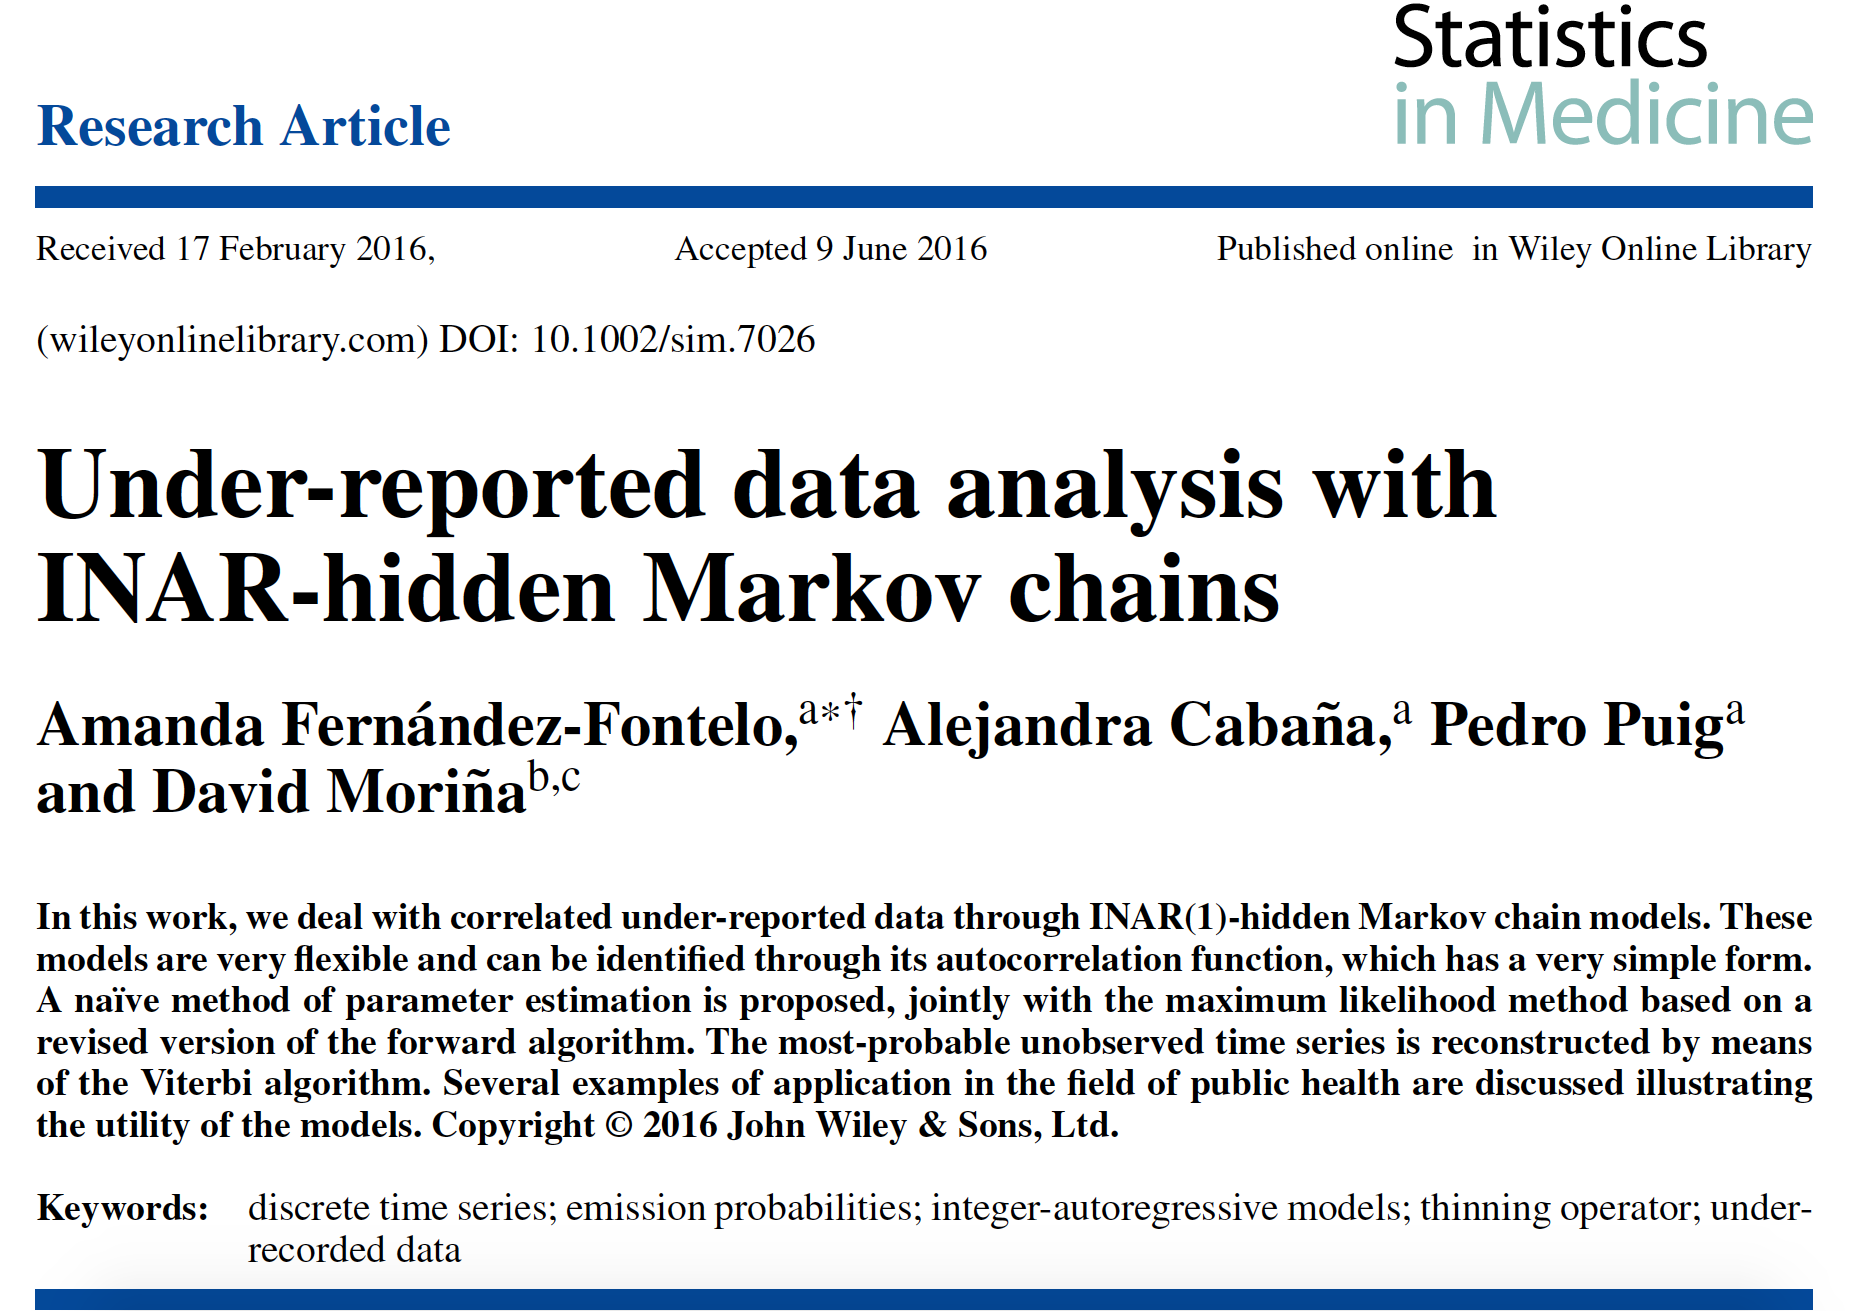
\includegraphics[scale=0.2]{SIM2016.png}
\end{frame}

\begin{frame}[fragile]{Modelo}
Un modelo similar se ha usado recientemente para evaluar la subnotificación de casos de diversas enfermedades como el virus del papiloma humano,
mesotelioma, botulismo, verrugas genitales o Covid-19 y fenómenos como la violencia de género

\centering

\includegraphics[scale=0.2]{bmc.png}
\end{frame}

\begin{frame}[fragile]{Modelo}
Un modelo similar se ha usado recientemente para evaluar la subnotificación de casos de diversas enfermedades como el virus del papiloma humano,
mesotelioma, botulismo, verrugas genitales o Covid-19 y fenómenos como la violencia de género

\centering
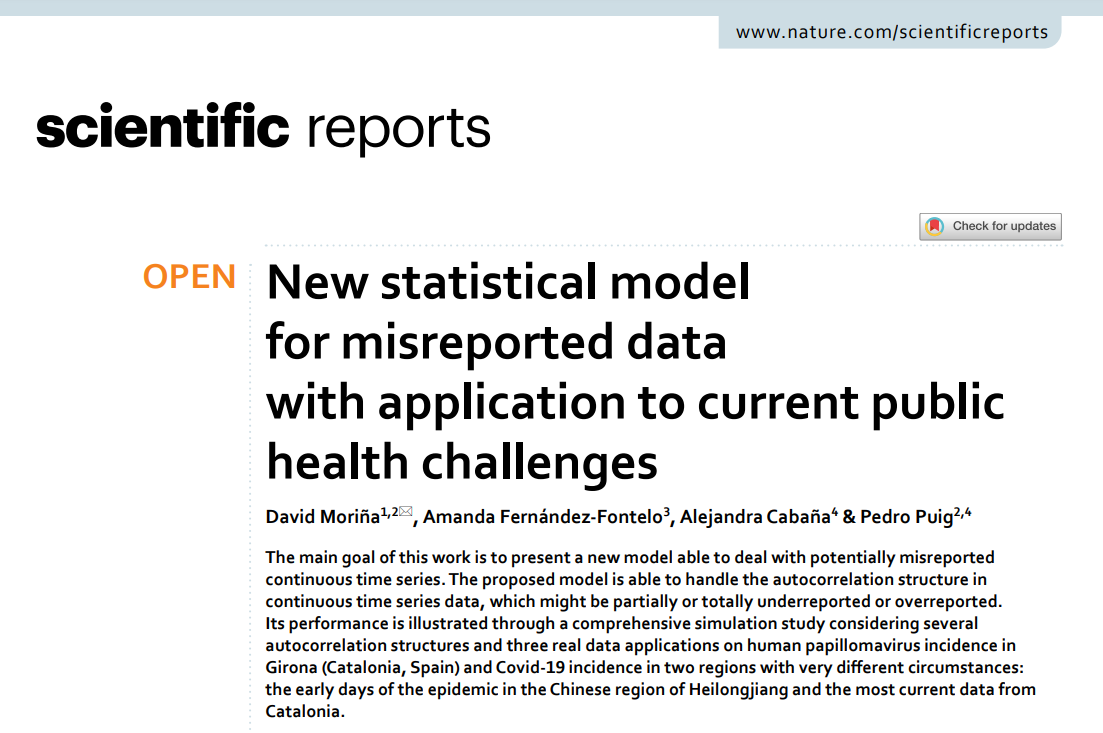
\includegraphics[scale=0.2]{sr.png}
\end{frame}

\begin{frame}[fragile]{Modelo}
Un modelo similar se ha usado recientemente para evaluar la subnotificación de casos de diversas enfermedades como el virus del papiloma humano,
mesotelioma o botulismo y fenómenos como la violencia de género

\centering
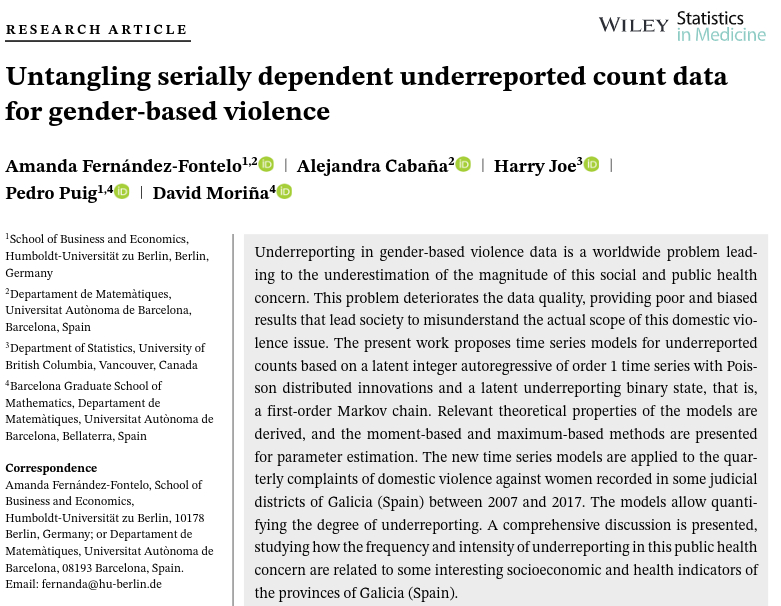
\includegraphics[scale=0.9]{SIM2019.jpg}
\end{frame}

\begin{frame}{Modelo}
\begin{itemize}
 \item Para evaluar la evolución del fenómeno en 2021 se desarrollará un modelo similar a los
anteriores pero que permita determinar también si ha habido un uso superior de los
servicios sanitarios en relación a los periodos de normalidad
 \item Para ello se desarrollará una modificación del thinning binomial de manera que
permita también que el resultado de la operación sea un valor mayor que el original
 \item Los nuevos modelos desarrollados en el marco de este proyecto se pondrán a disposición
de la comunidad científica y técnica de manera libre y gratuita en la forma de un
paquete para el conocido software estadístico R
\end{itemize}
\end{frame}

\begin{frame}[plain]
\centering

\includegraphics[width=0.7\textwidth ]{thanks.pdf}
\end{frame}

\end{document}
% \begin{frame}{Blocks}
%   Three different block environments are pre-defined and may be styled with an
%   optional background color.
% 
%   \begin{columns}[T,onlytextwidth]
%     \column{0.5\textwidth}
%       \begin{block}{Default}
%         Block content.
%       \end{block}
% 
%       \begin{alertblock}{Alert}
%         Block content.
%       \end{alertblock}
% 
%       \begin{exampleblock}{Example}
%         Block content.
%       \end{exampleblock}
% 
%     \column{0.5\textwidth}
% 
%       \metroset{block=fill}
% 
%       \begin{block}{Default}
%         Block content.
%       \end{block}
% 
%       \begin{alertblock}{Alert}
%         Block content.
%       \end{alertblock}
% 
%       \begin{exampleblock}{Example}
%         Block content.
%       \end{exampleblock}
% 
%   \end{columns}
% \end{frame}
% \begin{frame}{Math}
%   \begin{equation*}
%     e = \lim_{n\to \infty} \left(1 + \frac{1}{n}\right)^n
%   \end{equation*}
% \end{frame}
% \begin{frame}{Line plots}
%   \begin{figure}
%     \begin{tikzpicture}
%       \begin{axis}[
%         mlineplot,
%         width=0.9\textwidth,
%         height=6cm,
%       ]
% 
%         \addplot {sin(deg(x))};
%         \addplot+[samples=100] {sin(deg(2*x))};
% 
%       \end{axis}
%     \end{tikzpicture}
%   \end{figure}
% \end{frame}
% \begin{frame}{Bar charts}
%   \begin{figure}
%     \begin{tikzpicture}
%       \begin{axis}[
%         mbarplot,
%         xlabel={Foo},
%         ylabel={Bar},
%         width=0.9\textwidth,
%         height=6cm,
%       ]
% 
%       \addplot plot coordinates {(1, 20) (2, 25) (3, 22.4) (4, 12.4)};
%       \addplot plot coordinates {(1, 18) (2, 24) (3, 23.5) (4, 13.2)};
%       \addplot plot coordinates {(1, 10) (2, 19) (3, 25) (4, 15.2)};
% 
%       \legend{lorem, ipsum, dolor}
% 
%       \end{axis}
%     \end{tikzpicture}
%   \end{figure}
% \end{frame}
% \begin{frame}{Quotes}
%   \begin{quote}
%     Veni, Vidi, Vici
%   \end{quote}
% \end{frame}
% 
% {%
% \setbeamertemplate{frame footer}{My custom footer}
% \begin{frame}[fragile]{Frame footer}
%     \themename defines a custom beamer template to add a text to the footer. It can be set via
%     \begin{verbatim}\setbeamertemplate{frame footer}{My custom footer}\end{verbatim}
% \end{frame}
% }
